\documentclass[11pt]{article}
\usepackage[a4paper,left=22mm,right=22mm,top=23mm,bottom=25mm]{geometry}
\usepackage{graphicx}
\usepackage{url}
\usepackage{hyperref}
\usepackage{amsmath}
\usepackage{fancyhdr}
\usepackage[czech]{babel}
\usepackage[utf8]{inputenc}
\hypersetup{colorlinks=true,linkcolor=blue,urlcolor=blue}

\begin{document}
\clubpenalty 10000
\widowpenalty 10000

\title{1. Řešení problému batohu metodou hrubé síly a jednoduchou heuristikou}
\author{Ladislav Martínek}
\date{}
\maketitle
 
\section{Zadání úlohy} 


\begin{enumerate}
\item Naprogramujte řešení 0/1 \href{http://www.csc.kth.se/~viggo/wwwcompendium/node211.html#7374}{problému batohu} hrubou silou (tj. nalezněte skutečné optimum). Na zkušebních datech pozorujte závislost výpočetního času na n. 
\item Naprogramujte řešení problému batohu   heuristikou podle poměru cena/váha. Pozorujte

\begin{itemize}
\item závislost výpočetního času na n. Grafy jsou vítány (i pro exaktní metodu).
\item průměrnou a maximální relativní chybu (tj. zhoršení proti exaktní metodě) v závislosti na n.
\end{itemize}
\end{enumerate}  

\section{Rozbor možných variant řešení}

Problém batohu je zadán vstupními proměnnými, tedy vektorem hmotností a cen jednotlivých předmětů. Dále omezením, což je maximální hmotnost, kterou lze do batohu naložit. Konfigurační proměnná je binární vektor, který specifikuje zdali se předmět v batohu nachází (1) nebo nenachází (0). Formát výstupu je shodný s konfigurační proměnou.

Problém batohu lze řešit exaktně tzv. hrubou silou, pomocí které lze nalézt optimální řešení. Pro hledání optimálního řešení tedy vyzkoušíme všechny možné konfigurace obsahu batohu. Z této úvahy vyplývá, že je nutné vyzkoušet $2^n$ konfigurací, kde $n$ je počet předmětů, ze kterých lze vybírat. 

Dalším možným řešením problému batohu je řešením pomocí jednoduché heuristiky, která bere v úvahu poměr $\frac{\text{cena}}{\text{váha}}$. Objekty poté přidáváme do batohu v pořadí podle velikosti tohoto poměru. Poměr přesně určuje pořadí přidávání předmětů do batohu. Algoritmus s heuristikou je tedy deterministický. Při běhu je nutné provést počet kroků, který vychází z toho, že pro každý předmět spočítám poměr a~předměty podle poměru seřadím. Dále postupně zkouším každý předmět přidat do batohu v pořadí podle poměru. Algoritmus s touto heuristikou však nemusí nalézt vždy optimální řešení a~je závislý na vstupních parametrech. Existují tedy instance problému, pro které je bezchybný a takové instance, pro které vykazuje vysokou chybu.

\section{Rámcový popis postupu řešení}
Cílem úlohy bylo vyhodnotit časovou náročnost obou řešení, tedy jak metody hrubou silou, tak jednoduchou heuristikou. Problém hrubou silou jsem řešil rekurzivní metodou, protože je výhodný její komfortní a přehledný zápis. 

V rámci řešení tedy budu načítat jednotlivé soubory a z nich instance problému a každou instanci vyřeším. Při řešení budu měřit výkon a následně počítat relativní chybu pro každou instanci. Jednotlivá data budu ukládat do csv souborů.

\section{Popis kostry algoritmu}\label{kap:1}
Vytvořený algoritmus má dvě možné použití. První je $solve$, které vypíše optimální řešení pro daný problém. Druhý $stats$, který načítá problémy ze souboru nebo soubory s problémy z celé složky. Dále je pro každý problém spočítáno optimální a heuristické řešení. Při běhu je měřen CPU čas pomocí knihovny $timeit$. Pro nejmenší problémy je každé řešení vícenásobně opakováno a je vzata průměrná hodnota. Pro řešení větších problémů se počet opakování snižuje, protože při vyšším čase výpočtu instance již mezi opakováními nejsou téměř žádné rozdíly a vyhodnocování by trvalo příliš dlouhou dobu.

V řešení jsem také odřízl větve, kde již byla překročena maximální hmotnost.

V heuristickém řešení jsem nejprve spočítal jednotlivé poměry, které jsem seřadil. K seřazení jsem použil seřazenou mapu pro uchování indexu předmětu pro reprezentaci výsledku. Poté jsem postupně zkoušel přidávat předměty od toho s největším poměrem.

Na závěr jsem spočítal relativní chyby pro danou instanci problému $rel = \frac{c(OPT) - c(APX)}{c(OPT)}$. Data jsem ukládána po jednotlivých instancí. Průměrování jsem prováděl při tvorbě vizualizace, protože na těchto datech jednotlivých instancí lze počítat různé statistické ukazatele pro jednotlivé velikosti instancí.

\section{Experimenty}
\begin{figure}\centering
	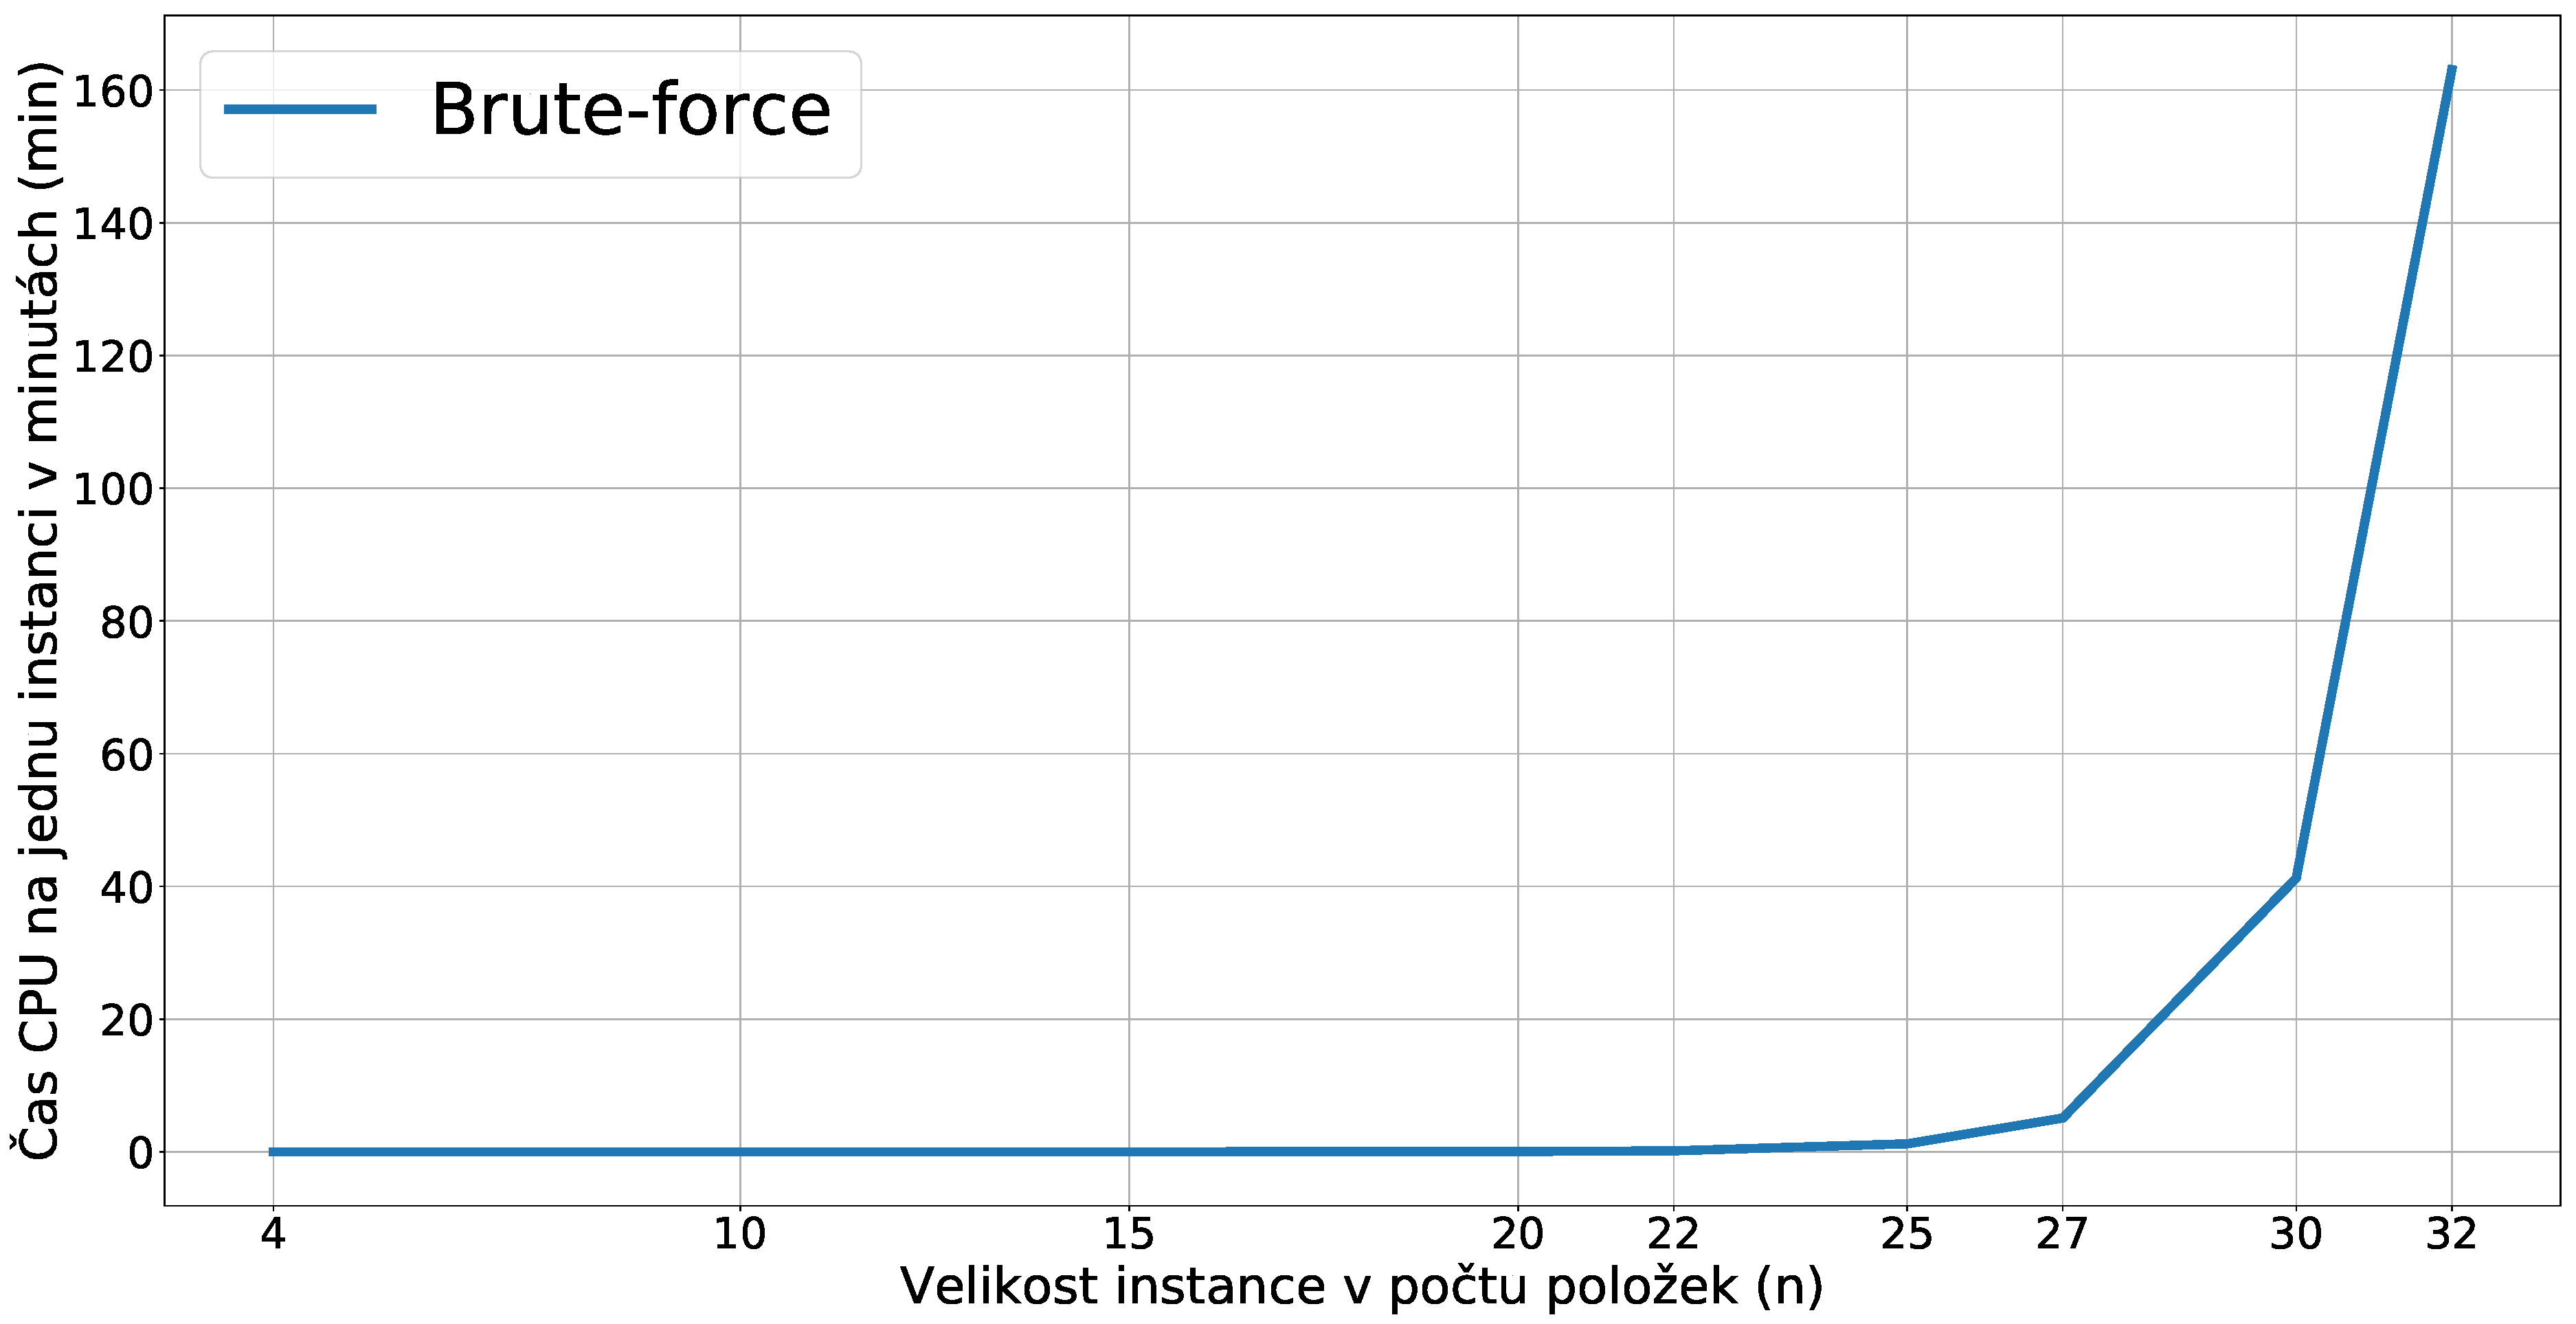
\includegraphics[scale=0.25]{img/1}
 	\caption[1]{Brute-force řešení. Časová náročnost.}\label{fig:1}
 \end{figure} 	
 \begin{figure}\centering
	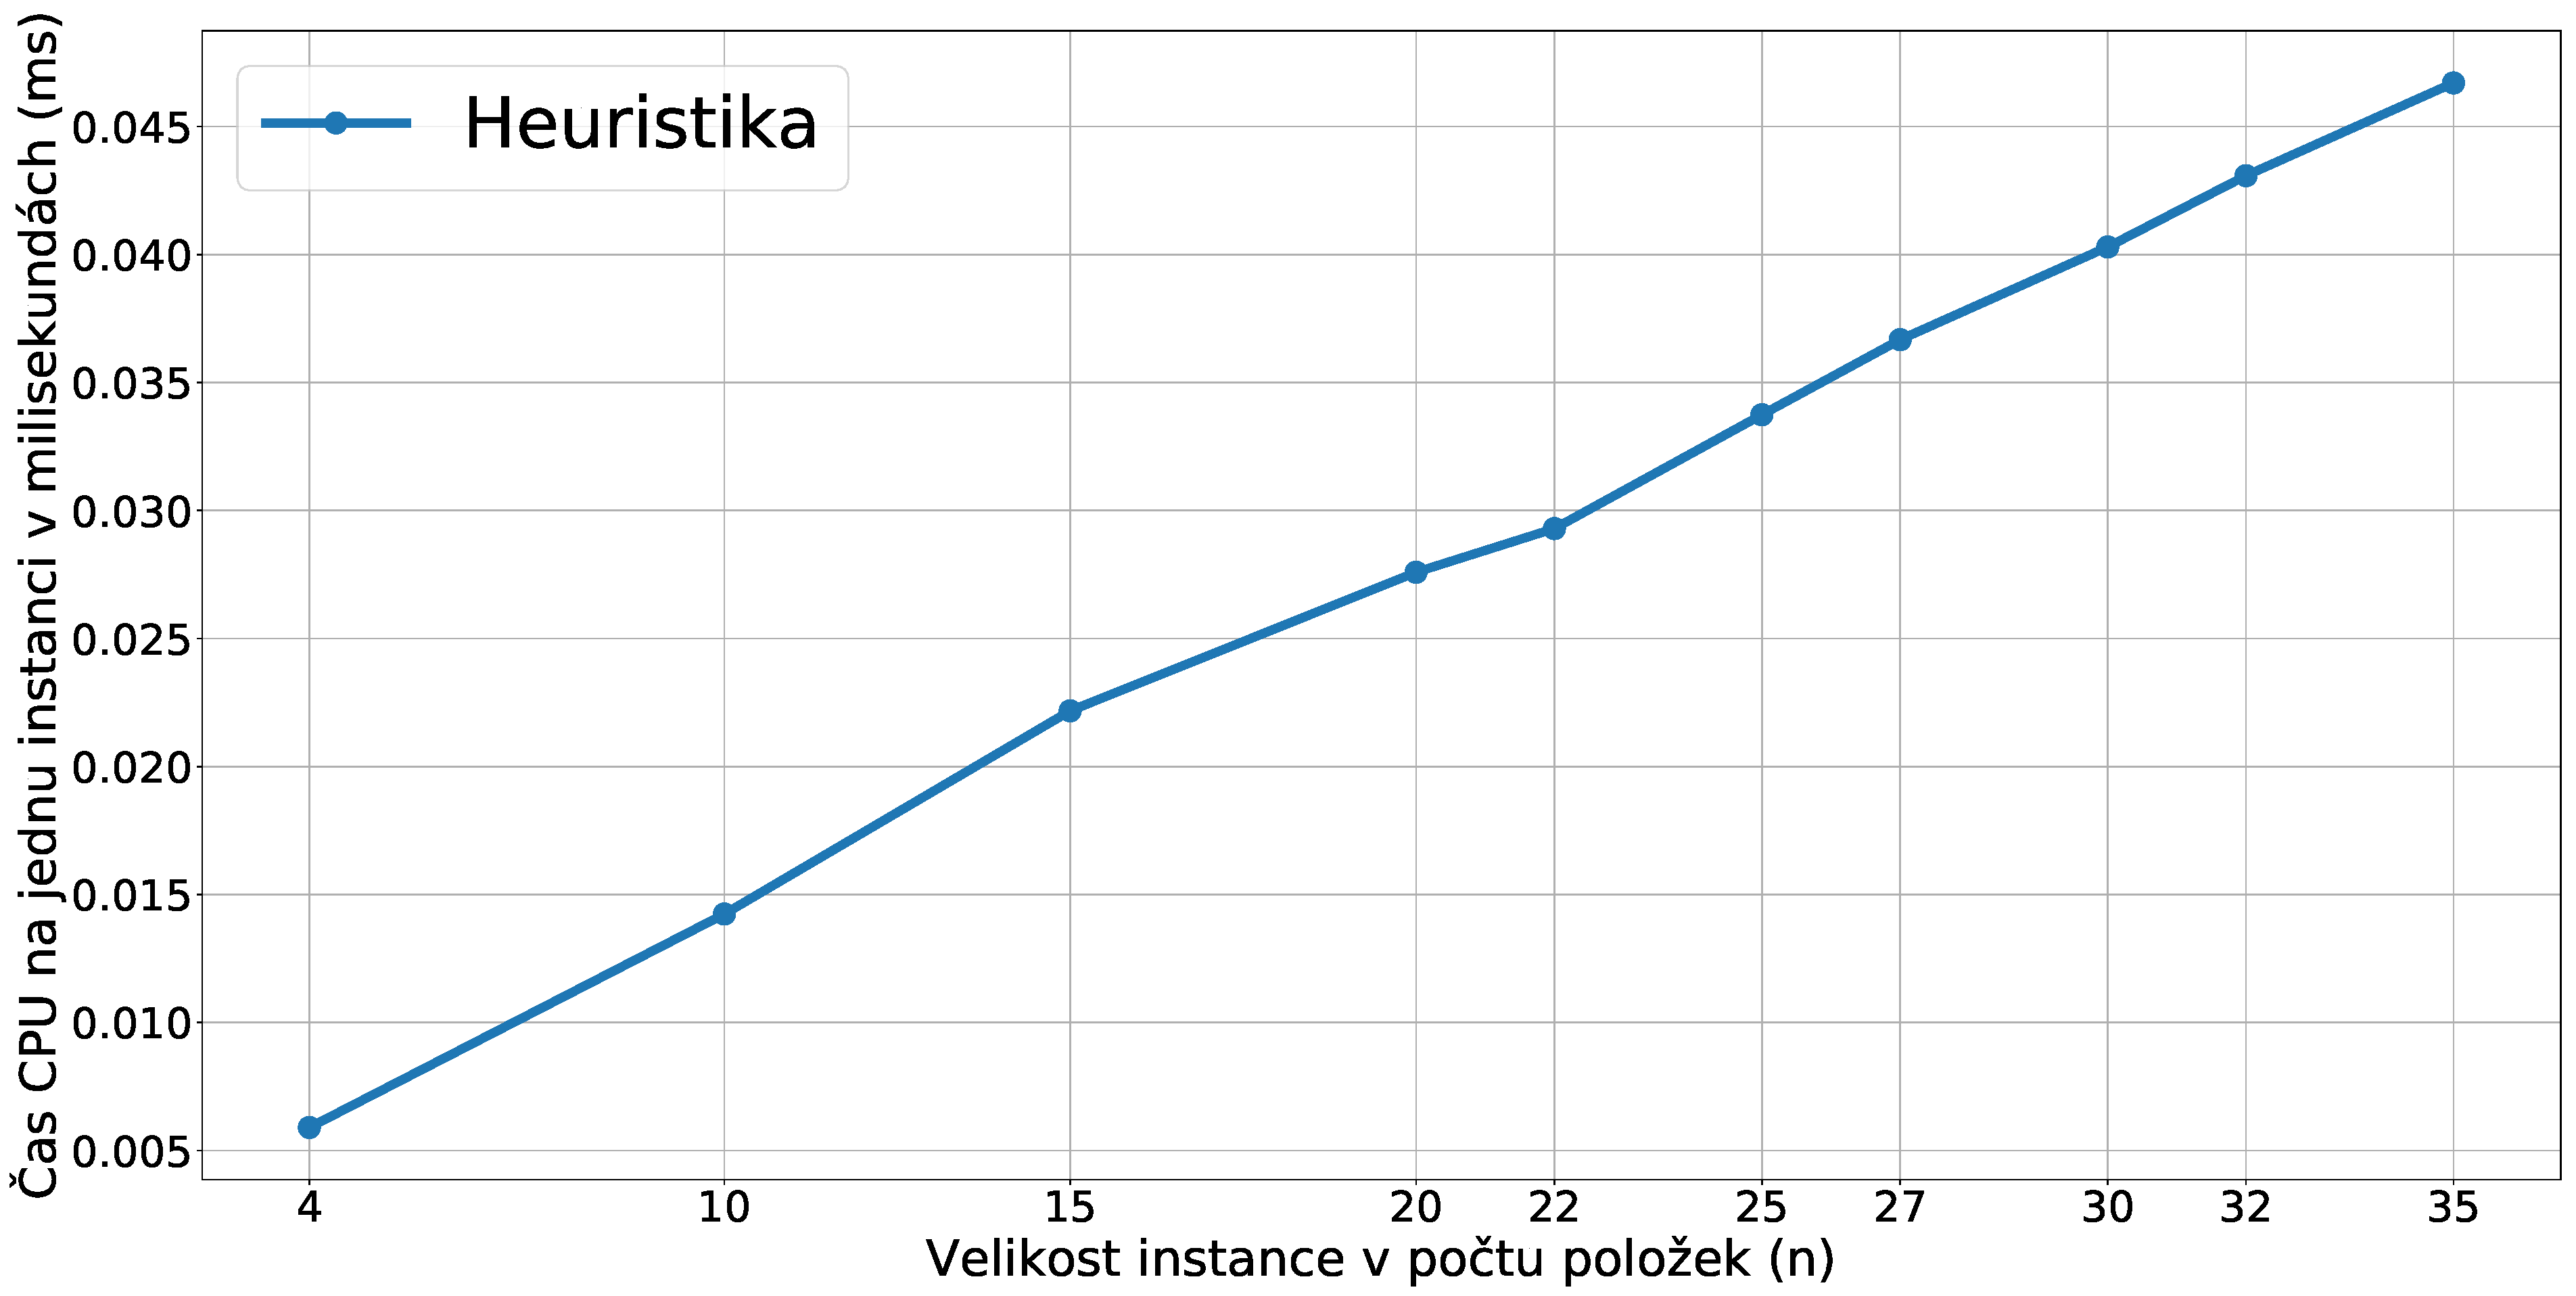
\includegraphics[scale=0.25]{img/2}
 	\caption[2]{Řešení pomocí heuristiky. Časová náročnost.}\label{fig:2}
 \end{figure} 	
 
Experimenty jsem prováděl v režimu jednoho vlákna na starším datovém serveru v podobě starého notebooku, který v době výpočtu nebyl používán. Výsledky tedy nejsou ovlivněny jinými běžícími programy. Procesor na testovacím stroji: \textit{Intel Pentium T3400 (2 cores). Taktován na 2.16~GHz s~1~MB cache}.
Měření času CPU probíhalo v knihovně $timeit$ s několika násobným průchodem pro menší instance.

Na grafu \ref{fig:1} můžeme vidět závislost výpočetního času metody hrubou silou na velikosti instance. Graf \ref{fig:1} ukazuje, že výpočetní náročnost je exponenciálně závislá na velikosti instance n. Křivka tedy přímo kopíruje exponenciálu. Graf tedy ukázal předpoklad z rozboru řešení. Na grafu je také vidět, že řešení jedné instance velikosti 32, trvalo průměrně kolem 160 minut. Z tohoto důvodu jsem skončil s řešení instance o velikosti 32. Toto omezení ale nemělo velký vliv, protože i~s~ním je exponencíální průběh jasně patrný.

Na obrázku \ref{fig:2} Můžeme vidět závislost výpočetního času medoty výpočtu pomocí heuristiky na velikosti instance. Na grafu \ref{fig:2} je vidět  téměř lineární závislost na velikosti vstupní instance n. Tato závislost je tedy ještě výnasobena $log(n)$ pro řadící algoritmus pro pole s poměry. Tento graf tedy opět potvrdil předpoklad.
\begin{figure}\centering
	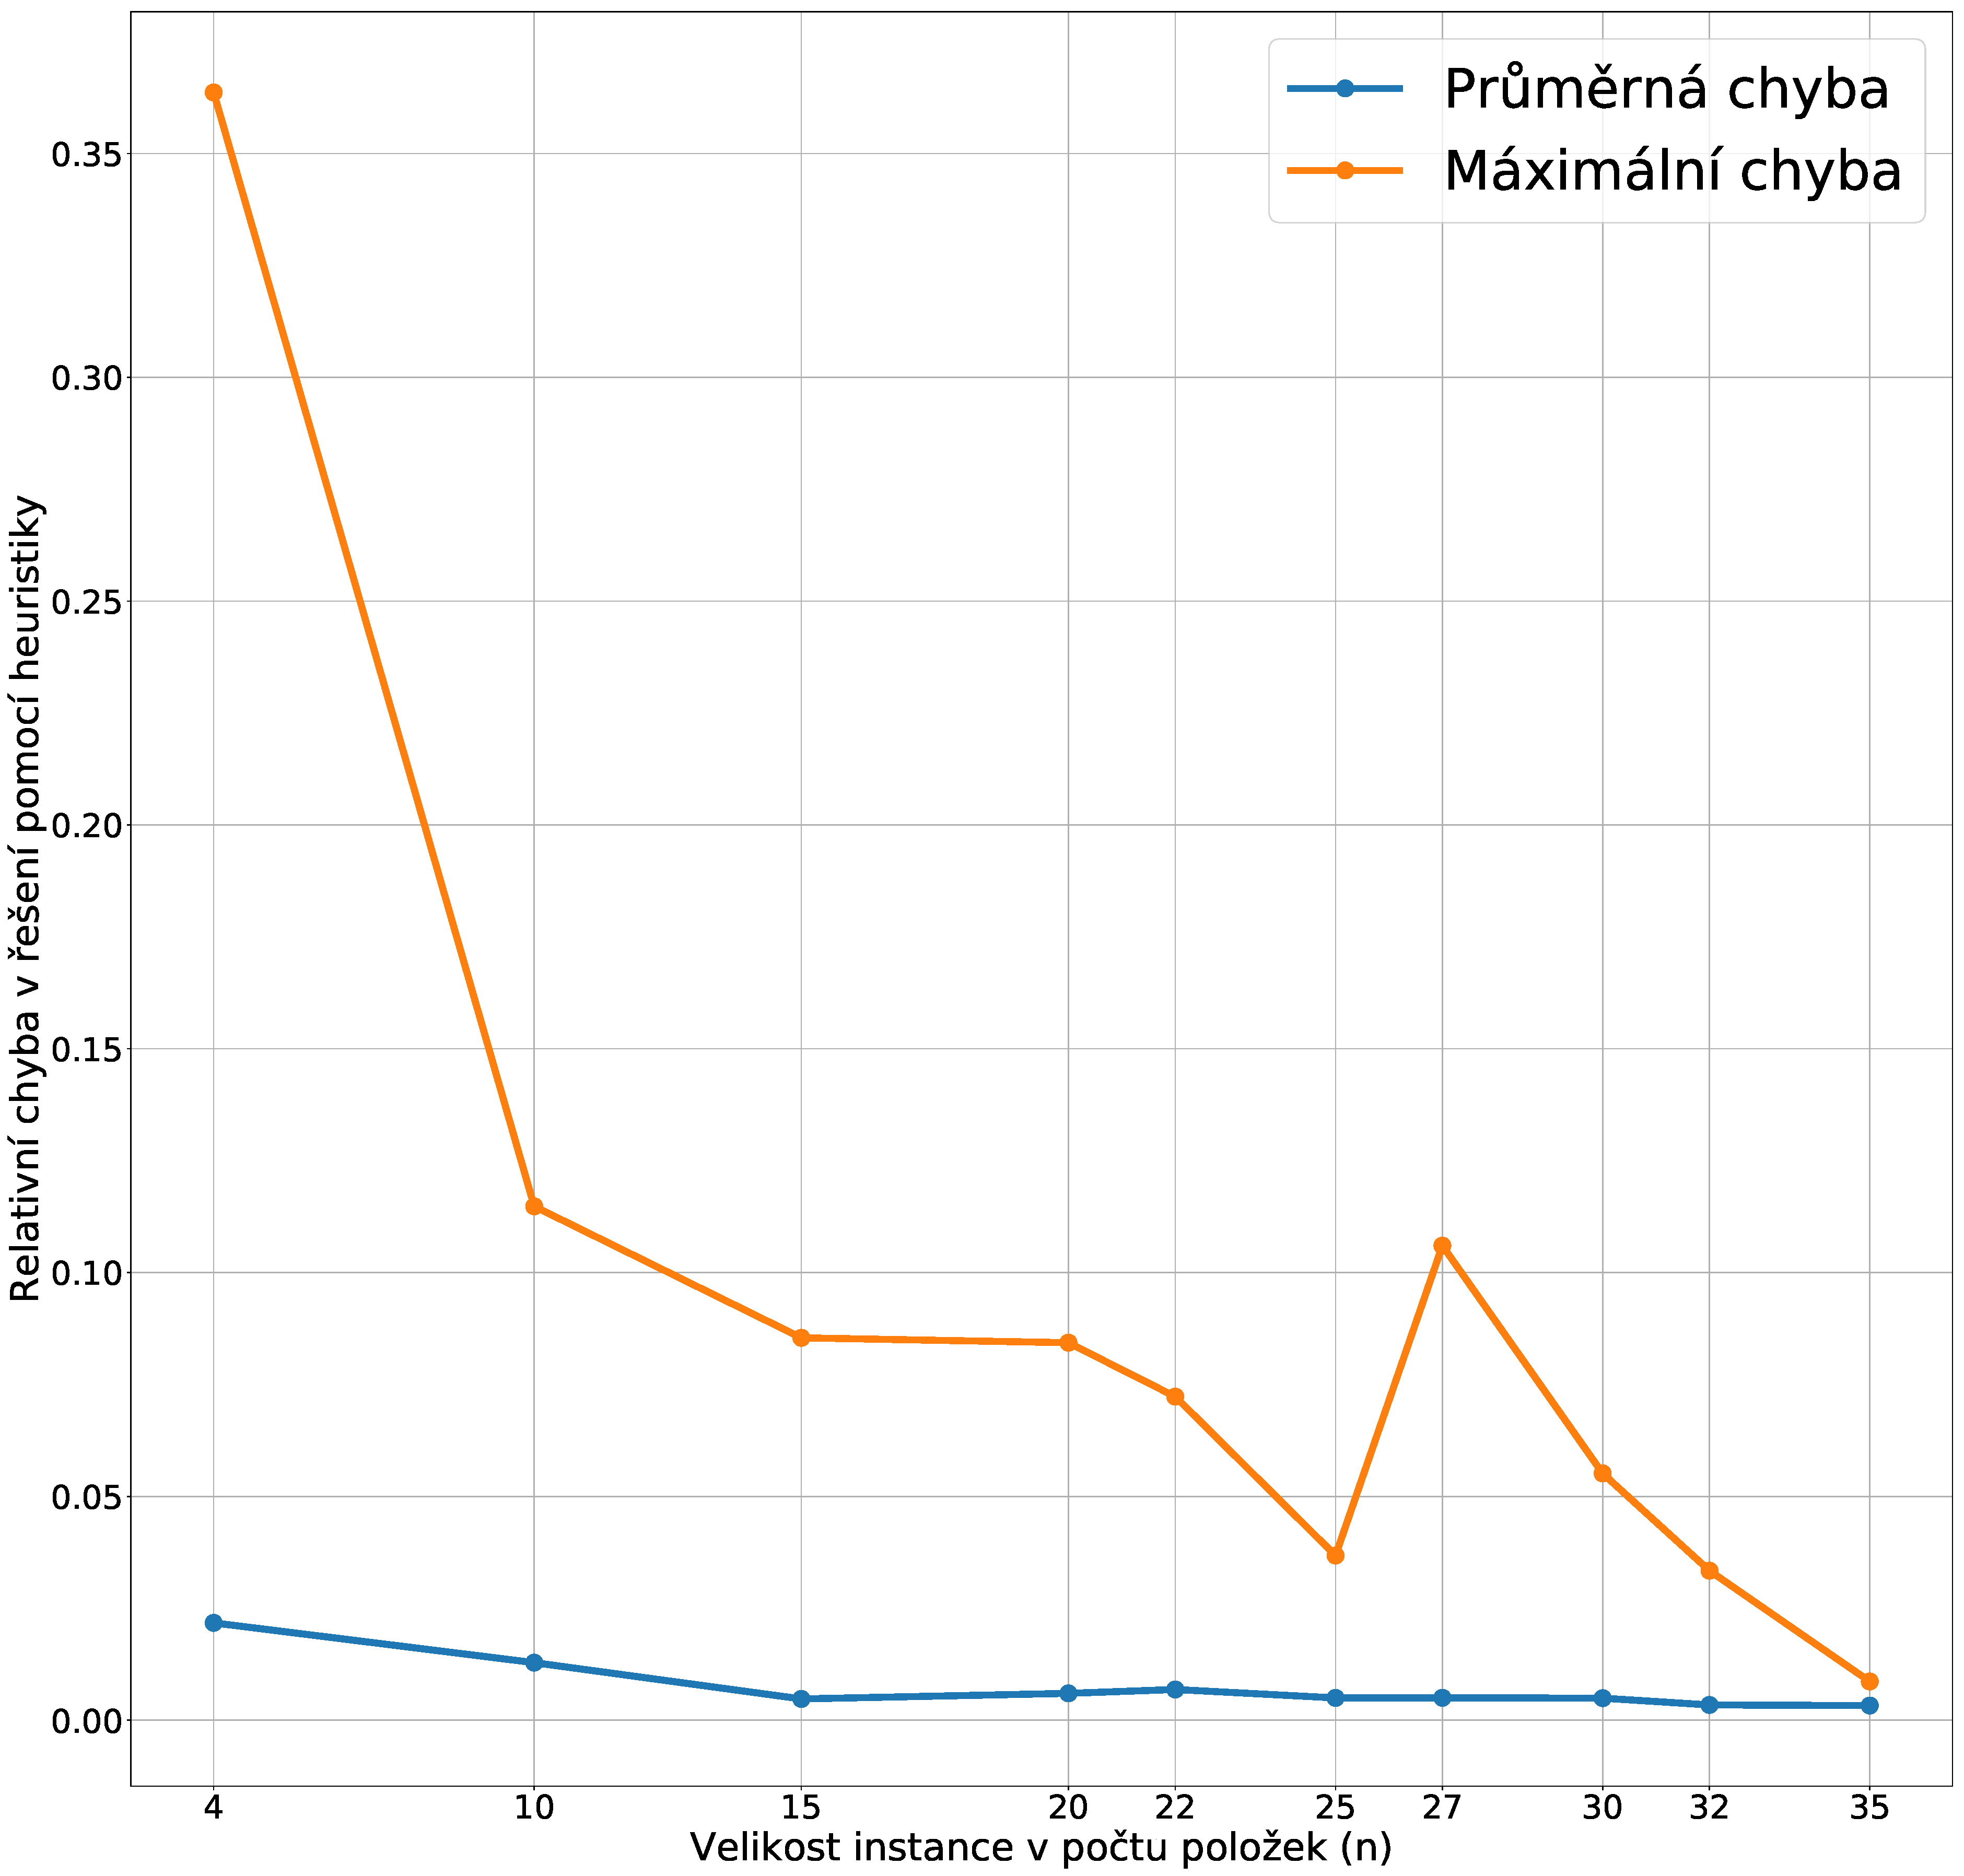
\includegraphics[scale=0.25]{img/3}
 	\caption[3]{Řešení pomocí heuristiky. Velikost relativní chyby.}\label{fig:3}
 \end{figure} 	
Měření relativní cyby jsem prováděl podle postupu popsaného v~kapitole~\ref{kap:1}. Na grafu \ref{fig:3} jsou zobrazeny křivky pro maximální a~průměrnou relativní chyby řešení pomocí heuristiky. Je jasně patrné, že chyba klesá se zvětšující se instancí. 

S zvětšující se instancí také klesá rozdíl mezi průměrnou a maximální chybou. Řešení pomocí heuristiky tedy může být využito k řešení velkých instancí, které nejsou upočitatelné metodou hrubé síly. Možnost menšího rozdílu mezi maximální a průměrnou chybou, která je patrná může být způsobena různými faktory. Například, že se již nevyskytují takové instance, pro které vykazuje onu vysokou chybu. Nebo také například, že pro takto velké instance je těžké tyto instance najít. 

 
\section{Závěr}
V průběhu experimetu jsme si prakticky ověřili předpoklady a řešení problému batohu pomocí hrubé síly a jednoduchou heuristikou. Rozdíl mezi těmito metodami se podle vykonaných experimentů snižuje s velikostí instance. Experimenty pro každé n byly vykonány na 50 instancích problému. Pokud instance byli generovány přijatelně náhodně je možné předpokládat, že by toto chování metody vykazovali i pro další instance. 

I přes předpoklad exponenciální složitosti mě při řešení nárůst výpočetního času překvapil a~s~využitím pomalejšího programovacího jazyka a staršího stroje, který složí již jen jako datový server, trvalo měření velice dlouho. 

Na druhou stranu mě pozitivně překvapila heuristika, která vykazovala minimální přůměřnou aproximační chybu a je tedy pro velké intance použitelná.

\end{document}